		\documentclass[12pt]{book}
\usepackage[a4paper, total={6in, 8in}]{geometry}
\usepackage{amssymb}
\usepackage{listings}
\usepackage{color}
\usepackage{graphicx}
\usepackage{subfig}
\usepackage{float}
\definecolor{mygrey}{gray}{.96} % Light Grey
\definecolor{BrickRed}{RGB}{120,0,0}


\def\xbf{\mathbf{x}}
\def\zbf{\mathbf{z}}
\def\xibf{\mathbf{\xi}}
\lstset{
	language=R,              % choose the language of the code ("language=Verilog" is popular as well)
   tabsize=3,							  % sets the size of the tabs in spaces (1 Tab is replaced with 3 spaces)
	basicstyle=\footnotesize,               % the size of the fonts that are used for the code
	numbers=left,                   % where to put the line-numbers
	numberstyle=\footnotesize,              % the size of the fonts that are used for the line-numbers
	stepnumber=1,                   % the step between two line-numbers. If it's 1 each line will be numbered
	numbersep=5pt,                  % how far the line-numbers are from the code
	backgroundcolor=\color{mygrey}, % choose the background color. You must add \usepackage{color}
	showspaces=false,              % show spaces adding particular underscores
	showstringspaces=false,        % underline spaces within strings
	showtabs=false,                % show tabs within strings adding particular underscores
	frame=single,	                 % adds a frame around the code
	tabsize=3,	                    % sets default tabsize to 2 spaces
	captionpos=b,                   % sets the caption-position to bottom
	breaklines=true,                % sets automatic line breaking
	breakatwhitespace=false,        % sets if automatic breaks should only happen at whitespace
	%escapeinside={\%*}{*)},        % if you want to add a comment within your code
	commentstyle=\color{BrickRed}   % sets the comment style
}

\begin{document}
\title{\textbf{Monte Carlo Simulation Lab}}	
\title{\textbf{Assignment-9}}
\author{Shalu Rungta\\(140123033)\\Department of Mathematics\\IIT Guwahati}
\date{April 12th, 2016}

\maketitle

\newpage
\begin{enumerate}
\item[Q 1]  Generate 10 sample paths for the standard Brownian Motion in the time interval [0, 5] using the recursion.\newline
$W(t_{i+1})=W(t_i)+\sqrt{t_{i+1} - t_i}. Z_{i+1}$\newline
with 5000 generated values for each of the paths where $Z_{i+1}$ $ \backsim $ $N(0,1)$ .Plot all the sample paths in a single figure. Also estimate $E[W(2)]$ and $E[W(5)]$ from the $10$ paths
that you have generated.\\
\end{enumerate}
\textbf{Solution:}

\noindent{Code for R}

\begin{lstlisting}
x=NULL;
y=NULL;
png("1.png");
for ( i in 1:10)
{
	n=rnorm(5000);
	a=5/5000;
	b=seq(from=0,to=5,by=0.001);
	w=NULL;
	w[1]=0;
	for( k in 1:5000)
	{
		w[k+1]=w[k]+sqrt(a)*n[k];
	}
	plot(b,w,col=i+3, blim=c(-5,5),type='l', main="Brownian Paths");
	par(new=TRUE);
	x[i]=w[2000];
	y[i]=w[5000];
}
print( cat("E[W[2]] = ",mean(x)));
print( cat("E[W[5]] = ",mean(y)));
\end{lstlisting}
\newpage
\textbf{OUTPUT:}
E[W[2]] = -0.1799204 \\ 
E[W[5]] = -0.2217755 \\

\begin{figure}[H]
	\centering
	\subfloat[Brownian motion]{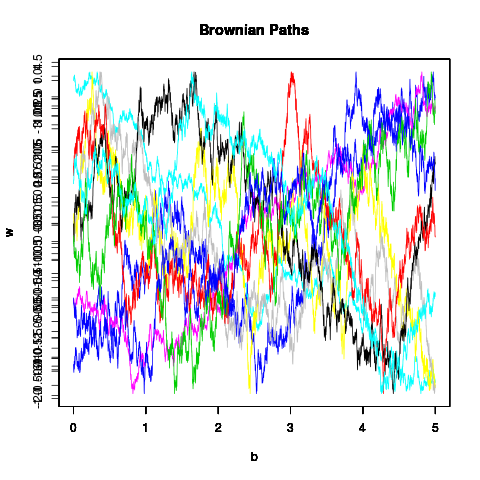
\includegraphics[width=0.6\textwidth]{1.png}}	
\end{figure}

\newpage


\begin{enumerate}
\item[Q 2] Repeat the above exercise with the following Brownian motion $(BM(\mu,\sigma ,2 ))$ discretization $X(t_{i=1}= X(t_i)= \mu(t_{i+1}-t_i) + \sigma \sqrt{t_{i+1}-t_i}. Z_{i+1} $ . Take $X(0)=5 , \mu= 0.06 $ and $ \sigma =0.3 $.\\

\end{enumerate}
\textbf{Solution:}

\noindent{Code for R}

\begin{lstlisting}
x=NULL;
y=NULL;
png("2.png");
for ( i in 1:10)
{
	n=rnorm(5000);
	a=5/5000;
	b=seq(from=0,to=5,by=0.001);
	w=NULL;
	w[1]=5;
	mu=0.06;
	rho=0.3;
	for( k in 1:5000)
	{
		w[k+1]=w[k]+mu*(a)+rho*sqrt(a)*n[k];
	}
	plot(b,w,col=i+3, blim=c(4,6),type='l', main="Brownian Paths");
	par(new=TRUE);
	x[i]=w[2000];
	y[i]=w[5000];
}
print( cat("E[W[2]] = ",mean(x)));
print( cat("E[W[5]] = ",mean(y)));
\end{lstlisting}
\newpage
The output of the code is:\\
E[W[2]] = 5.085238\\
E[W[5]] = 5.322875\\

\begin{figure}[H]
	\centering
	\subfloat[Brownian motion]{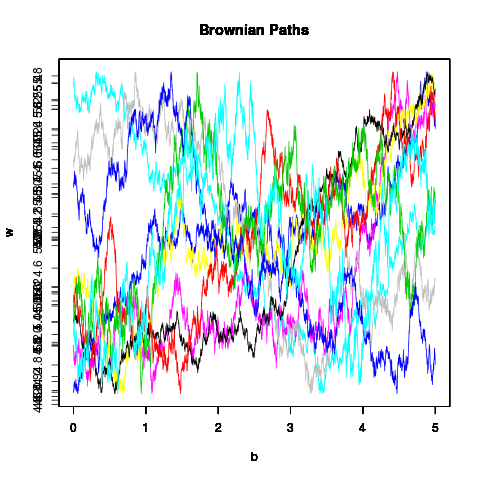
\includegraphics[width=0.6\textwidth]{2.png}}	
\end{figure}
\begin{enumerate}
\newpage
\item[Q 3]The Euler approximated recursion with time dependent $\mu$ and $\sigma$ is given by \newline
$Y(t_{i+1})= Y(t_i)+ \mu(t_i)(t_{i+1}- t_i) + \sigma(t_i) \sqrt{{t_{i+1}-t_i}}. Z_{i+1}$ \newline
Repeat the above exercise by taking \newline $Y(0)=5,\mu(t) = 0.0325-0.05t, \sigma(t)=0.012+0.0138t+0.00125t^2$\\
\end{enumerate}
\textbf{Solution:}

\noindent{Code for R}

\begin{lstlisting}
x=NULL;
y=NULL;
png("3.png");
for ( i in 1:10)
{
	n=rnorm(5000);
	a=5/5000;
	b=seq(from=0,to=5,by=0.001);
	w=NULL;
	w[1]=0;
	for( k in 1:5000)
	{
		
		rho=(0.012 + 0.0138*b[k]+0.00125*b[k]*b[k]);
		mu=(0.0325-0.05*b[k]);
		w[k+1]=w[k]+mu*(a)+rho*sqrt(a)*n[k];
	}
	plot(b,w,col=i+3, blim=c(-0.7,0.1),type='l', main="Brownian Paths");
	par(new=TRUE);
	x[i]=w[2000];
	y[i]=w[5000];
}
print( cat("E[W[2]] = ",mean(x)));
print( cat("E[W[5]] = ",mean(y)));
\end{lstlisting}
\newpage
The output of the code is:\\
E[W[2]] =  -0.02562826\\
E[W[5]] =  -0.4975501 

\begin{figure}[H]
	\centering
	\subfloat[Brownian motion]{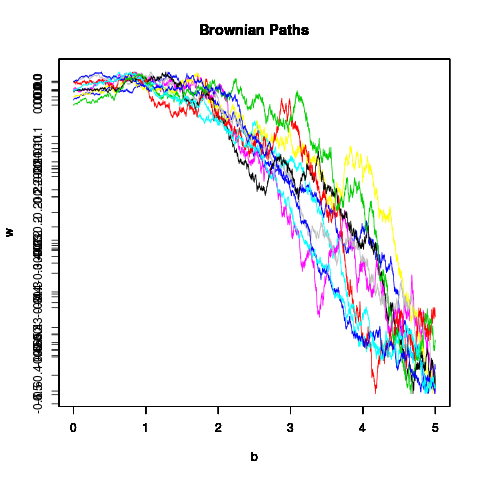
\includegraphics[width=0.6\textwidth]{3.png}}	
\end{figure}

\end{document}
